\newpage
\section{Frontend}\label{Frontend}
\subsection{Descrizione generale}\label{FeDescrizione}
L'architettura del front end pone come figura principale l'utente che interagisce con la piattaforma attraverso i componenti che costituiscono le schermate della stessa. Queste collaborano ed interagiscono a loro volta con le funzioni previste dai microservizi comunicando con il \glo{back end}.
\begin{figure}[H]
	\centering
	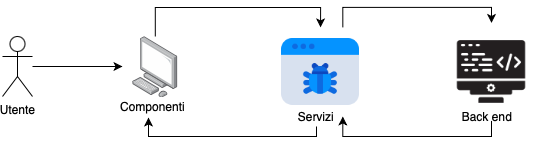
\includegraphics[scale=0.6]{Immagini/Frontend/fe.png}
	\caption{Architettura front end}
	\label{fig:fe}
\end{figure}
Attraverso l'utilizzo di Next.js, vengono utilizzati entrambi i tipi di pre-rendering dei dati: 
\begin{itemize}
	\item \textbf{Static generation:} il sistema genera le pagine \glo{HTML} a build time e vengono riusate ad ogni richiesta;
	\item \textbf{Server-side rendering:} il sistema genera le pagine HTML a ogni richiesta.
\end{itemize}
In \NomeProgetto\ vengono utilizzati i metodi:
\begin{itemize}
	\item \textbf{getStaticProps:} utilizzata per il data pre-fetching di tipo static genertion;
	\item \textbf{getServerSideProps:} utilizzata per il data pre-fetching di tipo server-side rendering.
\end{itemize}
\subsection{Diagramma dei package}
\begin{figure}[H]
	\centering
	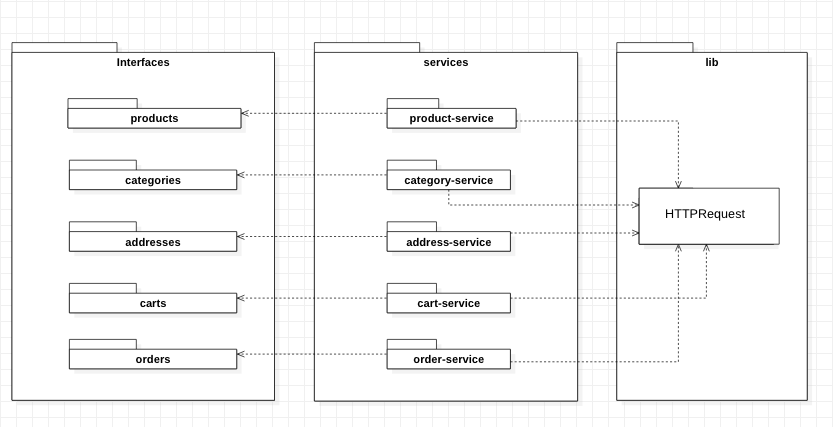
\includegraphics[scale=0.5]{Immagini/Frontend/DiagrammadeiPackage.png}
	\caption{Diagramma dei package}
	\label{fig:fe-packages}
\end{figure}
Il diagramma rappresenta le dipendenze tra le classi che individuano i \glo{microservizi}.
Il package \textbf{interfaces} contiene tutti i tipi che verranno utilizzati dal frontend.
La classe \textbf{HTTPRequest} è stata implementata per centralizzare le chiamate \glo{HTTP} e permettere il controllo dei tipi. Consiste in un wrapper della libreria nativa fetch e ridefinisce i metodi GET, POST, PATCH, PUT e DELETE. Ottiene la variabile d'ambiente contenente l'url del server dal file di configurazione relativo di dotenv, dal costruttore gli verrà passato l'url alla specifica \glo{API} il quale verrà aggiunto all'url precedente e su questo sarà possibile invocare i metodi precedentemente dichiarati.
Il package \textbf{services} rappresenta l'unico punto di collegamento tra i microservizi del backend e il frontend, tramite \glo{API} redatte utilizzando SwaggerHub, i vari servizi al suo interno andranno a invocare HTTPRequest per comunicare con il backend attraverso i metodi definiti.
I microservizi individuati e utilizzati per il frontend sono:
\begin{itemize}
	\item \textbf{Product;}
	\item \textbf{Address;}
	\item \textbf{Categories;}
	\item \textbf{Orders;}
	\item \textbf{Carts.}
\end{itemize}
\subsection{Services}\label{Services}
Ogni package presente all'interno del package services contiene il \glo{microservizio} che, invocando l'HTTPRequest, comunica con il back end. Ogni servizio contiene funzioni pubbliche asincrone e per questo motivo il tipo di ritorno è una \textbf{Promise<T>}.
\begin{figure}[H]
	\centering
	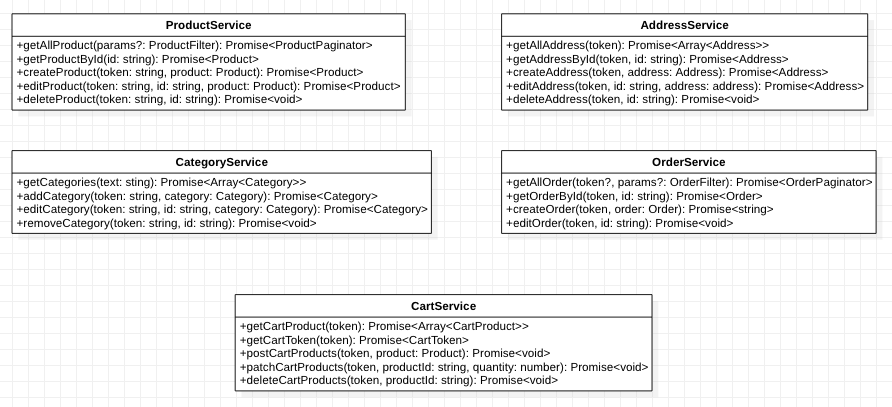
\includegraphics[scale=0.5]{Immagini/Frontend/ClassiService.png}
	\caption{Classi Service}
	\label{fig:feService}
\end{figure}
\newpage
\subsubsection{Esempio di funzionamento}\label{FeEsempio}
Di seguito si riporta il diagramma delle classi relativo al funzionamento del microservizio \textbf{product}. Come si può vedere è presente un'interfaccia ProductService che viene implementata dalla classe ProductServiceFetch e ogni suo metodo istanzia un oggetto HTTPRequest per l'API di interesse. È possibile implementare l'interfaccia ProductService diversamente rispetto a quanto rappresentato senza la necessità di modificare il codice utilizzatore, attraverso la modifica della variabile d'ambiente NEXT\_PUBLIC\_SERVICE\_METHOD sarà possibile scegliere quale implementazione utilizzare altrimenti verrà di default selezionata l'implementazione ProductServiceFetch. 
Per poter procedere con lo sviluppo della parte dei prodotti del frontend parallelamente con il backend, lo sviluppatore ha a disposizione la classe ProductServiceMock la quale ritornerà i dati predefiniti senza dover richiamare il server, basterà impostare la variabile NEXT\_PUBLIC\_SERVICE\_METHOD="mock".
\begin{figure}[H]
	\centering
	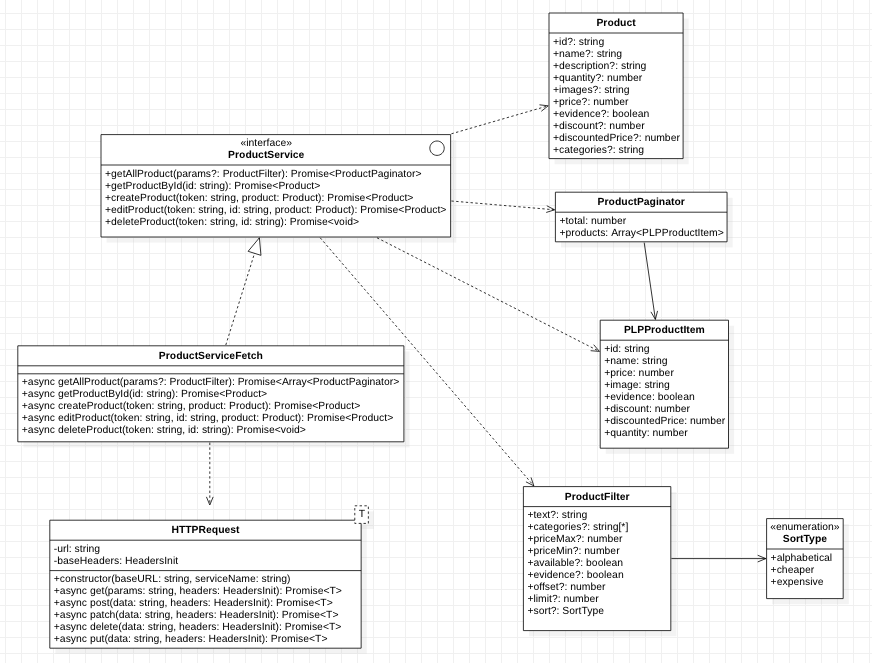
\includegraphics[width=\textwidth]{Immagini/Frontend/ProductService.png}
	\caption{Microservizio Product}
	\label{fig:fe-productservice}
\end{figure}